% !TeX TXS-program:compile = txs:///pythonlua

\documentclass[a4paper,11pt]{article}
\usepackage[pythontex,revgoku]{cp-base}
\graphicspath{{./graphics/}}
%variables
\donnees[%
	classe={1\up{ère} 2M2},
	matiere={[SPÉ.MATHS]},
	mois=Septembre,annee=2021,
	typedoc=EXOS~,
	numdoc=1,
	mois=Septembre,
	annee=2021
	]
%formatage
\author{Pierquet}
\title{\nomfichier}
\hypersetup{%
	pdfauthor={Pierquet},pdftitle={\nomfichier},allbordercolors=white,pdfborder=0 0 0,pdfstartview=FitH
	}
%divers
\lhead{\entete{\matiere}}
\chead{\entete{\lycee}}
\rhead{\entete{\classe{} - \mois{} \annee}}
\lfoot{\pied{\matiere}}
\cfoot{\logolycee{}}
\rfoot{\pied{\numeropagetot}}
\urlstyle{same}

\begin{document}
	
\pagestyle{fancy}

\part{CH01 - Polynômes du second degré - Exercices (Correction)}

\begin{clog}
Les captures d'écran ont été obtenues grâce au logiciel \cshell{Xcas}, et notamment sa version en ligne disponible à l'adresse \cshell{\url{https://www.xcasenligne.fr}}.

\smallskip

Cependant, les simplifications faites par le logiciel ne donnent pas forcément une écriture \og \uline{identique} \fg{} à celle trouvée à la main , donc \og prudence \fg{} !
\end{clog}

\exonum{0}%
\begin{enumerate}
	\item Pour la forme canonique, il s'agit de $a(x-\alpha)^2+\beta$ avec $\alpha=\dfrac{-b}{2a}$ et $\beta=a \times \alpha^2 + b \times \alpha + c$.
	\begin{center}
		\includegraphics[scale=0.3]{chap01_exos_corr_a}
	\end{center}
%	\begin{center}
%		\includegraphics[scale=0.5]{ch01_exos_corr_xcas_1}
%	\end{center}
	\item Pour déterminer le tableau de variation d'un trinôme, on utilise $\alpha$, $\beta$ puis l'\og ouverture \fg{} de la parabole :
	\begin{enumerate}
		\item $f(x)=2(x-4)^2+3$ est sous forme canonique :
		\begin{center}
			\begin{tikzpicture}
				\tkzTabInit{$x$/1,$f$/1.5}{$-\infty$,$4$,$+\infty$}
				\tkzTabVar{+/,-/$3$,+/}
			\end{tikzpicture}
		\end{center}
		\item $g(x)=-3(x+1)^2-5$ est sous forme canonique :
		\begin{center}
			\begin{tikzpicture}
				\tkzTabInit{$x$/1,$g$/1.5}{$-\infty$, $-1$, $+\infty$}
				\tkzTabVar{-/,+/$-5$,-/}
			\end{tikzpicture}
		\end{center}
		\item $h(x)=x(x-8)$ donne la forme canonique $h(x)=(x-4)^2-16$ :
		\begin{center}
			\begin{tikzpicture}
				\tkzTabInit{$x$/1,$h$/1.5}{$-\infty$, $4$, $+\infty$}
				\tkzTabVar{+/,-/$-16$,+/}
			\end{tikzpicture}
		\end{center}
	\end{enumerate}
	\item 
	\begin{enumerate}
		\item On a $f(x)=-2(x-2)^2-5$, et la parabole, \og non souriante \fg{}, a pour sommet $(2\,;\,-5)$.
		\item De ce fait, le maximum de $f$ est $M=-5$, atteint pour $x=2$.
	\end{enumerate}
\end{enumerate}

\medskip

\exonum{0} %exo2

\begin{enumerate}
	\item Pour résoudre les équations, on vérifie que ce sont des équations du 2\up{d} degré \og avec 0 de l'autre côté \fg{}, et si besoin on \og transforme \fg{} :
	\begin{itemize}
		\item on calcule $\Delta=b^2-4ac$ ;
		\item suivant son signe on a :
		\begin{itemize}
			\item aucune racine (et aucune factorisation) si $\Delta < 0$ ;
			\item une racine ($\nicefrac{-b}{2a}$) si $\Delta=0$ ;
			\item deux racines ($\nicefrac{(-b\pm \sqrt{\Delta})}{2a}$) si $\Delta > 0$.
		\end{itemize}
	\end{itemize}
	\begin{center}
		\includegraphics[scale=0.3]{chap01_exos_corr_b}
	\end{center}
	\item Pour écrire un trinôme sous forme factorisée, on calcule ses éventuelles racines (via $\Delta$) puis :
	\begin{itemize}
		\item factorisation $a(x-x_1)(x-x_2)$ si $\Delta>0$ ;
		\item factorisation $a(x-x_0)^2$ si $\Delta=0$ ;
		\item pas de factorisation si $\Delta<0$.
	\end{itemize}
	\begin{center}
		\includegraphics[scale=0.3]{chap01_exos_corr_c}
	\end{center}
%	\begin{center}
%		\includegraphics[scale=0.5]{ch01_exos_corr_xcas_5}
%	\end{center}
\end{enumerate}

\medskip

\exonum{0} %exo3

\medskip

On détermine les formes canoniques pour déterminer les tableaux de variations, et donc la courbe correspondante !
\begin{itemize}
	\item \textcolor{blue}{$f_1(x)=-x^2+2x-3=-(x-1)^2-2$ avec le sommet en $(1\,;\,-2)$}.
	\item \textcolor{red}{$f_2(x)=x^2+x+3=(x+0,5)^2+2,75$ avec le sommet en $(-0,5\,;\,2,75)$}.
	\item \textcolor{purple}{$f_3(x)=2x^2-5x+3=-2(x-1,25)^2-0,125$ avec le sommet en $(1,25\,;\,-0,125)$}.
	\item \textcolor{ForestGreen}{$f_4(x)=-2x^2-5x+3=-2(x+1,25)^2+6,125$  avec le sommet en $(-1,25\,;\,6,125)$}.
	\item \textcolor{orange}{$f_5(x)=x^2+x+\dfrac14=(x+0,5)^2$ avec le sommet en $(-0,5\,;\,0)$}.
\end{itemize}

\begin{center}
	\includegraphics[scale=0.3]{chap01_exos_corr_d}
\end{center}

%\begin{center}
%	\includegraphics[scale=0.5]{ch01_exos_corr_xcas_6}
%\end{center}

\begin{center}
	\tunits{1}{0.5}
	\tdefgrille{-5}{5}{1}{1}{-6}{7}{1}{1}
	\begin{tikzpicture}[x=\xunit cm,y=\yunit cm]
		%AXES & GRILLES
		\tgrilles[line width=0.4pt,color=lightgray] ;
		\axestikz ;
		\axextikz[size=\small]{-5,-4,...,4} ;
		\axeytikz[size=\small]{-6,-5,...,6} ;
		%LABELS
		\draw (5,2) node[right] {\blue $f_1(x)=-x^2+2x-3$} ;
		\draw (5,1) node[right] {\red $f_2(x)=x^2+x+3$} ;
		\draw (5,0) node[right] {\textcolor{purple}{$f_3(x)=2x^2-5x+3$}} ;
		\draw (5,-1) node[right] {\textcolor{ForestGreen}{$f_4(x)=-2x^2-5x+3$}} ;
		\draw (5,-2) node[right] {\textcolor{orange}{$f_5(x)=x^2+x+\tfrac14$}} ;
		%COURBES
		\clip (\xmin,\ymin) rectangle (\xmax,\ymax) ;
		%		\psplot[linewidth=1.5pt,linecolor=blue]{-5}{5}{-x^2+2*x-3}
		%		\psplot[linewidth=1.5pt,linecolor=red]{-5}{5}{x^2+x+3}
		%		\psplot[linewidth=1.5pt,linecolor=purple]{-5}{5}{2*x^2-5*x+3}
		%		\psplot[linewidth=1.5pt,linecolor=ForestGreen]{-5}{5}{-2*x^2-5*x+3}
		%		\psplot[linewidth=1.5pt,linecolor=orange]{-5}{5}{x^2+x+0.25}
		\draw[line width=1.5pt,blue,domain=-5:5,samples=200] plot(\x,{-\x*\x+2*\x-3});
		\draw[line width=1.5pt,red,domain=-5:5,samples=200] plot(\x,{\x*\x+\x+3});
		\draw[line width=1.5pt,purple,domain=-5:5,samples=200] plot(\x,{2*\x*\x-5*\x+3});
		\draw[line width=1.5pt,ForestGreen,domain=-5:5,samples=200] plot(\x,{-2*\x*\x-5*\x+3});
		\draw[line width=1.5pt,orange,domain=-5:5,samples=200] plot(\x,{\x*\x+\x+0.25});
	\end{tikzpicture}
\end{center}

\medskip

\exonum{2} %exo4

\begin{enumerate}
	\item Pour résoudre les équations suivantes, on les \textbf{transforme} pour se ramener à une équation que l'on sait résoudre :
	\begin{enumerate}
		\item L'équation proposée ne peut pas (encore) être résolue (pb avec le \og $x^3$ \fg), on transforme !
		
		$x^3-8x^2+18x=0 \ssi x(x^2-8x+18)=0$ qui est une \textbf{équation produit} :
		
		\hspace{5mm}$\bullet~~x=0$ ou
		
		\hspace{5mm}$\bullet~~x^2-8x+18=0$ pour lequel $\Delta=-8$ donc pas de solution pour cette \og partie \fg
		
		Ainsi $\mathscr{S}= \left\lbrace \strut 0 \right\rbrace$.
		\item Pour la deuxième équation, on va utiliser le \textbf{produit en croix}, et on a une valeur interdite ($x=-1$).
		
		$\dfrac{x^2+2x+1}{x+1}=2x-1 \ssi x^2+2x+1 = (2x-1)(x+1) \ssi x^2+2x+1 = 2x^2+x-1 \ssi -x^2+x+2 = 0$.
		
		On a $\Delta=9$ et les deux racines sont $x_1=2$ et $x_2=-1$ (valeur interdite !).
		
		Ainsi $\mathscr{S}= \left\lbrace \strut 2 \right\rbrace$.
		\item $\dfrac{3x^2+10x+8}{x+2}=2x+5 \ssi 3x^2+10x+8 = (x+2)(2x+5) \ssi 3x^2+10x+8=2x^2+9x+10$
		
		$\phantom{\dfrac{3x^2+10x+8}{x+2}=2x+5} \ssi x^2+x-2=0$ (avec $x \neq -2$).
		
		On a $\Delta=9$ et les deux racines sont $x_1=1$ et $x_2=-2$ (valeur interdite !).
		
		Ainsi $\mathscr{S}= \left\lbrace \strut 1 \right\rbrace$.
	\end{enumerate}
	\begin{center}
		\includegraphics[scale=0.3]{chap01_exos_corr_e}
	\end{center}
%	\begin{center}
%		\includegraphics[scale=0.5]{ch01_exos_corr_xcas_3}
%	\end{center}
	\item 
	\begin{enumerate}
		\item L'équation admet une seule racine (double) dans le cas où le discriminant est nul.
		
		Et $\Delta = 0 \ssi b^2-4ac = 0 \ssi (-4)^2 - 4 \times 1 \times (m-1) = 0 \ssi 16-4m+4 = 0 \ssi -4m = -20 \ssi m=5$.
		\item Dans ce cas, la racine (double) vaut $x_0=\dfrac{-b}{2a}=\dfrac{-(-4)}{2 \times 1} = 2$ (c'est l'identité remarquable $x^2-4x+4$ !)
	\end{enumerate}
	\item 
	\begin{enumerate}
		\item 2 est solution de l'équation car $2^2-5 \times 2 + 6 = 4 - 10 + 6 =0$.
		\item La somme des racines vaut $\nicefrac{-b}{a} = 5$ et le produit des racines vaut $\nicefrac{c}{a}=-6$.
		\item On a donc $x_1=2$ et donc $x_1 + x_2 = 5 \Rightarrow x_2 = 5 - 2 =3$.
	\end{enumerate}
	\item 
	\begin{enumerate}
		\item $\begin{dcases} x+y=18 \\xy=65 \end{dcases} \Rightarrow x$ et $y$ sont les racines de $X^2-18X+65$.
		
		On utilise $\Delta$, et on trouve $x=13$ et $y=5$ (ou le contraire\dots)
		\item $\begin{dcases} x+y=4 \\xy=5 \end{dcases} \Rightarrow x$ et $y$ sont les racines de $X^2-4X+5$.
		
		On utilise $\Delta$, et on ne trouve aucune solution\dots
	\end{enumerate}
\end{enumerate}

\medskip

\exonum{2} %exo5

\medskip

On pose $x$ le côté du premier carré, de sorte qu'on cherche $x$ tel que $x^2+(x+1)^2+(x+2)^2=15\,125 $

Et $x^2+(x+1)^2+(x+2)^2=15\,125 \ssi \dots \ssi 3x^2 + 6x-15\,150 = 0$ qui donne $x=70$ (l'autre solution est négative !).

\smallskip

De même, on cherche $x$ tel que $3x^2+6x-15\,122=0$ qui ne donne aucune solution entière !

\medskip

\exonum{2} %exo6

\medskip

On détermine :
\begin{itemize}
	\item l'aire totale du drapeau : $\mathscr{A}_T=4 \times 3=12$ ;
	\item l'aire de la croix : $\mathscr{A}_C = \text{(bde horiz)} + \text{(bde vert)} - \text{(petit carré du milieu en double)} = x \times 4 + x \times 3 - x^2 = -x^2+7x$. 
\end{itemize}
On cherche donc $x$ ($x\pg 0$) tel que $\mathscr{A}_C = 6 \ssi -x^2+7x = 6 \ssi -x^2+7x-6=0$.

On obtient $\Delta = 25$ et la solution (positive) $x=1$ (l'autre vaut $-6$ !)

Donc la bande doit avoir une largeur de 1~m.

\medskip

\exonum{2} %exo7

\begin{pyconcode}
# Calcul de alpha et de beta
from math import *
def analysetrinome(a,b,c):
	alpha = -b/(2*a)
	beta = a*alpha**2 + b*alpha + c
	print(f"Le sommet de la parabole a pour coordonnées ({alpha},{beta})")
	if a > 0 :
		print("La parabole est ouverte vers le haut")
	else :
		print("La parabole est ouverte vers le bas")

\end{pyconcode}

\begin{tcpythoncodeno}[15cm]
	\begin{pyverbatim}[][fontsize=\footnotesize,numbers=none]
		def analysetrinome(a,b,c) :
			alpha = -b/(2*a)
			beta = a*alpha**2 + b*alpha + c
			print(f"Le sommet de la parabole a pour coordonnées ({alpha},{beta})")
			if a > 0 :
				print("La parabole est ouverte vers le haut")
			else :
				print("La parabole est ouverte vers le bas")
	\end{pyverbatim}
\end{tcpythoncodeno}

On peut vérifier sur \cshell{\url{https://python.cpierquet.fr/?from=examples/2m2chap01exos.py}} :

\begin{consolepython}[15cm]
\begin{pyconsole}[][framesep=3mm,frame=single,label={[\scriptsize Début de la console \logopython]\scriptsize Fin de la console \logopython},fontsize=\footnotesize,framerule=1pt,rulecolor=\color{ForestGreen}]
analysetrinome(-1,2,-3)
\end{pyconsole}
\end{consolepython}
\end{document}